\documentclass[class = article,border = 5pt]{standalone}

\usepackage[usenames,dvipsnames]{xcolor}

\usepackage{tikz}
\usetikzlibrary{arrows, shapes, fit, backgrounds, calc}

\usepackage{amsmath, amsfonts, amsthm, amssymb}

\pgfdeclarelayer{background}
\pgfsetlayers{background,main}

\setlength{\parskip}{0pt}
\setlength{\parindent}{0pt}

\begin{document}

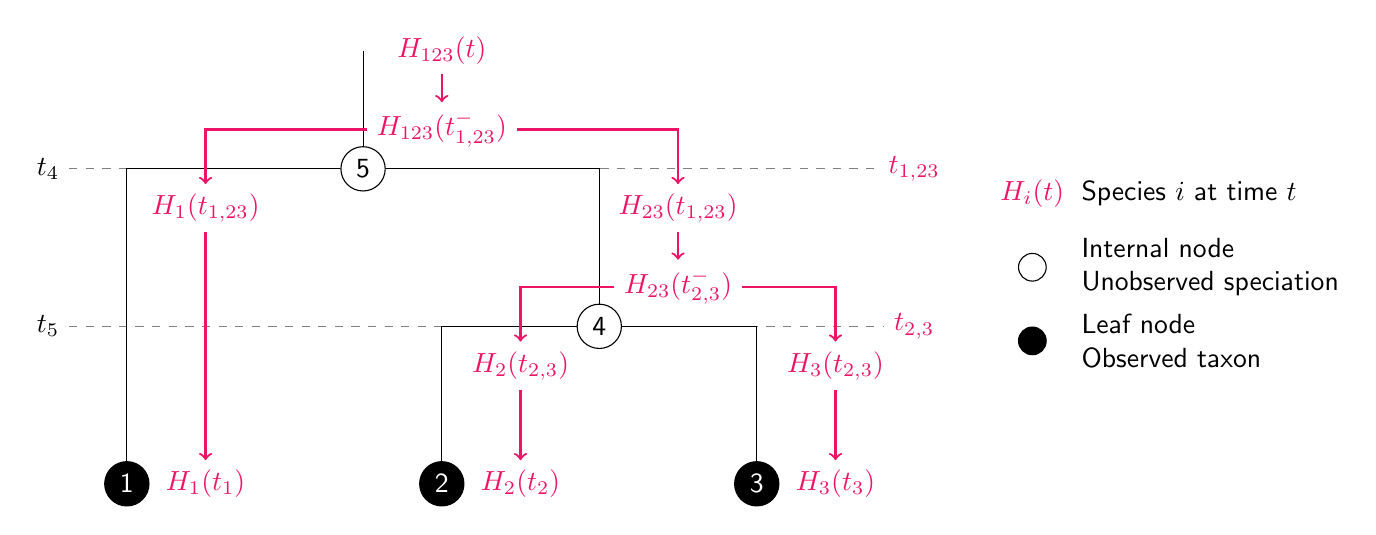
\begin{tikzpicture}

% Sans-serif text
\sffamily

% Set node and arrow styles for sets
\tikzset{Ht/.style={color = WildStrawberry}}
\tikzset{HtA/.style={color = WildStrawberry, thick, ->}}

% Tree node styles
\tikzset{nS/.style={draw, shape = circle, inner sep = 1pt, minimum width = 16pt}}
\tikzset{inS/.style={nS, fill = white}}
\tikzset{lnS/.style={nS, fill = black, text = white}}

% Tree nodes
\node (n1) [lnS] at (-4,2) {1};
\node (n2) [lnS] at (0, 2) {2};
\node (n3) [lnS] at (4, 2) {3};

\path let \p1 = (n2), \p2 = (n3) in node (n4) [inS] at ($ (0.5*\x1 + 0.5*\x2, 4) $) {4};
\path let \p1 = (n4), \p2 = (n1) in node (n5) [inS] at ($ (0.5*\x1 + 0.5*\x2, 6) $) {5};

\node (n0) at ($ (n5) + (0, 1.5) $) {};

% Placeholder nodes
\path let \p1 = (n5), \p2 = (n4) in node (p54) at (\x2, \y1) {};
\path let \p1 = (n5), \p2 = (n1) in node (p51) at (\x2, \y1) {};

\path let \p1 = (n4), \p2 = (n2) in node (p42) at (\x2, \y1) {};
\path let \p1 = (n4), \p2 = (n3) in node (p43) at (\x2, \y1) {};

% Edges
\draw[black] (n0.center) -- (n5);

\draw[black] (n5) -| (n4);
\draw[black] (n5) -| (n1);

\draw[black] (n4) -|(n3);
\draw[black] (n4) -| (n2);

% Set nodes
\node (h123t) [Ht] at ($ (n0) + (1, 0) $) {$ H_{123}(t) $};
\node (h123t5m) [Ht] at ($ (n5) + (1, 0.5) $) {$ H_{123}(t_{1,23}^-) $};

\node (h1t5) [Ht] at ($ (p51) + (1, -0.5) $) {$ H_1(t_{1,23}) $};
\node (h1t1) [Ht] at ($ (n1) + (1, 0) $) {$ H_1(t_1) $};

\node (h23t5) [Ht] at ($ (p54) + (1, -0.5) $) {$ H_{23}(t_{1,23}) $};
\node (h23t4m) [Ht] at ($ (n4) + (1, 0.5) $) {$ H_{23}(t_{2,3}^-) $};

\node (h2t4) [Ht] at ($ (p42) + (1, -0.5) $) {$ H_2(t_{2,3}) $};
\node (h2t2) [Ht] at ($ (n2) + (1, 0) $) {$ H_2(t_2) $};

\node (h3t4) [Ht] at ($ (p43) + (1, -0.5) $) {$ H_3(t_{2,3}) $};
\node (h3t3) [Ht] at ($ (n3) + (1, 0) $) {$ H_3(t_3) $};

% Set arrows
\draw[HtA] (h123t) -- (h123t5m);

\draw[HtA] (h123t5m) -| (h1t5);
\draw[HtA] (h123t5m) -| (h23t5);

\draw[HtA] (h23t5) -- (h23t4m);
\draw[HtA] (h23t4m) -| (h2t4);
\draw[HtA] (h23t4m) -| (h3t4);

\draw[HtA] (h1t5) -- (h1t1);
\draw[HtA] (h2t4) -- (h2t2);
\draw[HtA] (h3t4) -- (h3t3);

% Background image
\begin{pgfonlayer}{background}

	% Time nodes
    \path let \p1 = ($ (n1) + (-1, 0) $), \p2 = (n4) in node (t2a) at (\x1, \y2) {$ t_5 $};
	\path let \p1 = ($ (h3t3) + (1, 0) $), \p2 = (n4) in node (t2b) [color = WildStrawberry] at (\x1, \y2) {$ t_{2,3} $};

	\path let \p1 = (t2a), \p2 = (n5) in node (t5a) at (\x1, \y2) {$ t_4 $};
	\path let \p1 = (t2b), \p2 = (n5) in node (t5b) [color = WildStrawberry] at (\x1, \y2) {$ t_{1,23} $};

	% Time lines
	\draw[black!50, dashed] (t5a) -- (t5b);
	\draw[black!50, dashed] (t2a) -- (t2b);

\end{pgfonlayer}

% Event labels
\path let \p1 = (t5b), \p2 = (n0), \p3 = (n3) in node (hl) [Ht] at ($ (\x1, 0.67*\y2 + 0.33*\y3) + (1.5, 0) $) {$ H_i(t) $};
\path let \p1 = (t5b), \p2 = (n0), \p3 = (n3) in node (il) [inS, minimum size = 10pt] at ($ (\x1, 0.5*\y2 + 0.5*\y3) + (1.5, 0) $) {};
\path let \p1 = (t5b), \p2 = (n0), \p3 = (n3) in node (ll) [lnS, minimum size = 10pt] at ($ (\x1, 0.33*\y2 + 0.67*\y3) + (1.5, 0) $) {};

\node [align = left, anchor = west] at ($ (hl) + (0.5, 0) $) {Species $ i $ at time $ t $};
\node [align = left, anchor = west] at ($ (il) + (0.5, 0) $) {Internal node \\ Unobserved speciation};
\node [align = left, anchor = west] at ($ (ll) + (0.5, 0) $) {Leaf node \\ Observed taxon};

\end{tikzpicture}

\end{document}
